\documentclass[12pt,letterpaper]{memoir}
    % memoir commands to define the text block geometry
    \setulmarginsandblock{0.5in}{*}{*}
    \setlrmarginsandblock{0.5in}{*}{*} % leave space in left margin for punched holes

\usepackage{xparse}
\usepackage{blindtext}
\usepackage{enumitem}
\usepackage{graphicx}

\usepackage{amsmath,mathtools,amssymb}
% See https://texblog.net/latex-archive/maths/amsmath-matrix/ 
% for an explanation of this extention of the amsmath matrix commands.
% It's a way to enable "augmented matrices" using a new optional argument:
%
% \begin{pmatrix}[cc|c]
%     1 & 2 & 3\\
%     4 & 5 & 9
%   \end{pmatrix}
%
\makeatletter
\renewcommand*\env@matrix[1][*\c@MaxMatrixCols c]{%
  \hskip -\arraycolsep
  \let\@ifnextchar\new@ifnextchar
  \array{#1}}
\makeatother

\usepackage{bm} % bold math package

\usepackage{booktabs}
\usepackage{multirow}
\usepackage{hyperref}
\usepackage{systeme}

\usepackage{tcolorbox}
    \tcbuselibrary{skins}
    \tcbuselibrary{raster}
    \tcbuselibrary{skins}
\usepackage{tikz}
    \usetikzlibrary{arrows.meta}
\usepackage{tkz-base}
\usepackage{tkz-fct}    
\usepackage{pgfplots}
    \pgfplotsset{compat=newest}

% for inserting blanks that the students fill in
\usepackage{dashundergaps} % for \gap
\dashundergapssetup{
    teacher-mode=false, % set to true to show answers 
    gap-format=underline,
    teacher-gap-format=underline,
    gap-font={\ECFAugie\MTversion{augie}\color{black}},
    gap-numbers=false,
    gap-widen=true,
    gap-extend-percent=100, % note: making this too big might create errors
    gap-number-format=\,\textsuperscript{\normalfont(\thegapnumber)},
}

\usepackage{emerald}
\usepackage[subdued]{mathastext}% no italic for Augie anyhow
    \MTDeclareVersion[n]{lmvtt}{T1}{lmvtt}{m}{n}
    \MTfamily{augie}
    \Mathastext[augie]

    \dashundergapssetup{
        gap-format=underline,
        teacher-gap-format=dot,
        gap-font={\ECFAugie\MTversion{augie}\color{black}},
        gap-numbers=false,
        gap-widen=true,
        gap-extend-percent=75, % note: making this too big might create errors
        gap-number-format=\,\textsuperscript{\normalfont(\thegapnumber)},
    }
    \newcommand{\myEmph}{\bfseries\itshape}
\newcommand{\myClassName}{{\tagged{pre-AP}{pre-AP }}Algebra 2}

% So I can save/restore \fboxsep
\newlength{\mySavedFboxsep}
\newcommand{\mySaveFboxsep}{\setlength{\mySavedFboxsep}{\fboxsep}}
\newcommand{\mySaveAndSetFboxsep}[1]{
    \setlength{\mySavedFboxsep}{\fboxsep}
    \setlength{\fboxsep}{#1}
}
\newcommand{\myRestoreFboxsep}{\setlength{\fboxsep}{\mySavedFboxsep}}

% A centered tcolorbox
%
% #1 - options to pass to tcolorbox
%
\NewDocumentEnvironment{myCenteredBox}{m}{%
    \begin{center}
    \begin{tcolorbox}[#1]
}{
    \end{tcolorbox}
    \end{center}
}


% A centered system of equations
%
\NewDocumentCommand{\myCenteredSysteme}{m}{%
    \begin{center}\systeme{#1}\end{center}
}

%
% This specialized command is my way of typesetting a table for
% students to use when solving systems of equations using matrices.
%
% - I make it really wide, because I need horizontal space. The increase in margin width 
%   is adjustable, but frankly, there are a lot of hard-coded dimensions in the table, so
%   I'm not positive that generality works well.
%
% - I put the content in a tikz picture with an OPAQUE background, since I 
%   plan to overlay this on top of Examples, which have dotted boxes around 
%   them at the "normal" margins.
%
% - The table uses the multirow package so that I can have the "Solution" box span two cells.
%
\NewDocumentCommand{\myWideMatrixTable}{O{-0.7in}}{
    \begin{adjustwidth}{#1}{#1}
        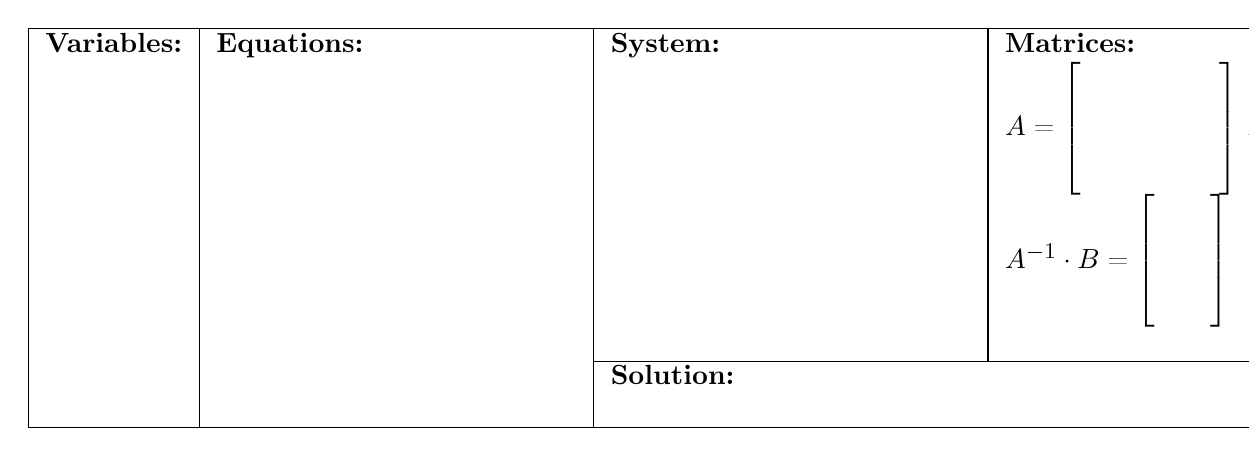
\begin{tikzpicture}
            \node
            [
                text width=1.25\textwidth, %I dinked with the multiplier to get balanced margins
                fill=white!30, 
                fill opacity=1,
                text opacity=1,
                inner sep=0pt,
            ]
            {%
                \begin{tabular}{|l|m{1.8in}|m{1.8in}|m{2.1in}|}
                    \hline
                    {\bfseries\scshape Variables:} & {\bfseries\scshape Equations:} & {\bfseries\scshape System:} & {\bfseries\scshape Matrices:} \\
                    % & & & \\
                    & & & 
                    \(
                        A = 
                        \begin{bmatrix}
                            \phantom{99} & \phantom{99} & \phantom{99} \\
                            \phantom{99} & \phantom{99} & \phantom{99} \\
                            \phantom{99} & \phantom{99} & \phantom{99} \\
                            \phantom{99} & \phantom{99} & \phantom{99} \\
                        \end{bmatrix}
                    \)
                    \(
                        B = 
                        \begin{bmatrix}
                            \phantom{999}\\
                            \phantom{999}\\
                            \phantom{999}\\
                            \phantom{999}\\
                    \end{bmatrix}
                    \)
                    \\
                    & & &
                    \(
                        A^{-1}\cdot B = 
                        \begin{bmatrix}
                            \phantom{9999}\\
                            \phantom{999}\\
                            \phantom{999}\\
                            \phantom{999}\\
                    \end{bmatrix}
                    \)
                    \\
                    & & & \\ \cline{3-4}
                    & & 
                    \multicolumn{2}{l|}{\bfseries\scshape Solution:}
                    \\ 
                    & & 
                    \multicolumn{2}{l|}{\,}
                    \\ 
                    \hline
                \end{tabular}
            };
        \end{tikzpicture}
    \end{adjustwidth}
}

    \usepackage{xparse}
\usepackage{blindtext}
\usepackage{enumitem}
\usepackage{graphicx}

\usepackage{amsmath,mathtools,amssymb}
% See https://texblog.net/latex-archive/maths/amsmath-matrix/ 
% for an explanation of this extention of the amsmath matrix commands.
% It's a way to enable "augmented matrices" using a new optional argument:
%
% \begin{pmatrix}[cc|c]
%     1 & 2 & 3\\
%     4 & 5 & 9
%   \end{pmatrix}
%
\makeatletter
\renewcommand*\env@matrix[1][*\c@MaxMatrixCols c]{%
  \hskip -\arraycolsep
  \let\@ifnextchar\new@ifnextchar
  \array{#1}}
\makeatother

\usepackage{bm} % bold math package

\usepackage{booktabs}
\usepackage{multirow}
\usepackage{hyperref}
\usepackage{systeme}

\usepackage{tcolorbox}
    \tcbuselibrary{skins}
    \tcbuselibrary{raster}
    \tcbuselibrary{skins}
\usepackage{tikz}
    \usetikzlibrary{arrows.meta}
\usepackage{tkz-base}
\usepackage{tkz-fct}    
\usepackage{pgfplots}
    \pgfplotsset{compat=newest}

% for inserting blanks that the students fill in
\usepackage{dashundergaps} % for \gap
\dashundergapssetup{
    teacher-mode=false, % set to true to show answers 
    gap-format=underline,
    teacher-gap-format=underline,
    gap-font={\ECFAugie\MTversion{augie}\color{black}},
    gap-numbers=false,
    gap-widen=true,
    gap-extend-percent=100, % note: making this too big might create errors
    gap-number-format=\,\textsuperscript{\normalfont(\thegapnumber)},
}

\usepackage{emerald}
\usepackage[subdued]{mathastext}% no italic for Augie anyhow
    \MTDeclareVersion[n]{lmvtt}{T1}{lmvtt}{m}{n}
    \MTfamily{augie}
    \Mathastext[augie]

% ---------------------------------------------------------------------------
% number lines using Tkz
% ---------------------------------------------------------------------------

% a simple number line
%
% #1 scale of the numberline
% #2 max x
% #3 min x (optional, if absent it defaults to negative of the max)
% #4 label on the x-axis (optional, if absent there's no label)
%
\NewDocumentCommand{\myNumberLine}{ O{0.4} m o O{{}} }{
    \begin{tikzpicture}[
        scale=#1,
        xaxe style/.style = { very thick, arrows={-{Straight Barb}}, },                 
        ]
        \tkzInit[ xmax=#2, xmin=\IfValueTF{#3}{#3}{-#2}, xstep=1, ]
        \tkzDrawX[
            % right=12pt,
            label=#4,
            noticks=false, % Yes, I want ticks!
            tickup=1em, tickdn=1em,
            right space=0.05cm, left space=0.05cm, % extend the line beyond the last ticks
            ]
        % \tkzLabelX[ 
        %     % orig=false,
        %     step=#4,
        %     font=\small,
        %     below left=2pt,
        %  ]
    \end{tikzpicture}
}


% ---------------------------------------------------------------------------
% x-y graphs using Tkz
% ---------------------------------------------------------------------------

% a tikzpicture wrapper environment that uses Tkz to draw an x-y grid
%
% #1 tikzpicture scale
%
% #2 optional xmin (defaults to negative of xmax)
% #3 xmax
% #4 optional ymin (defaults to negative of ymax)
% #5 ymax
%
\NewDocumentEnvironment{myTikzpictureGrid}{ m omom }{
    \begin{tikzpicture}[
        scale=#1,
        xaxe style/.style = { dashed, very thick, arrows={-{Straight Barb}}, },                 
        yaxe style/.style = { dashed, very thick, arrows={-{Straight Barb}}, },                 
        ]
        \tkzInit[
            xmin={\IfValueTF{#2}{#2}{-#3}}, xmax=#3, xstep=1,
            ymin={\IfValueTF{#4}{#4}{-#5}}, ymax=#5, ystep=1,
            ]
        \tkzGrid[ sub, subxstep=1, subystep=1, ]
        \tkzDrawX[label={$x$},color=black, right=0.2em,]
        \tkzDrawY[label={$y$},color=black, above=0.2em,]
        % \tkzLabelX[orig=false,] \tkzLabelY[orig=false,]
}{
    \end{tikzpicture}
}

% A counter to number the problems in the guided notes.
\newcounter{MyProblemCounter}
\setcounter{MyProblemCounter}{1}
\newcommand{\useMyProblemCounter}{\theMyProblemCounter\stepcounter{MyProblemCounter}}


% the style to use to render the problem counter on paper
\newcommand{\myProblemFont}{\bfseries\itshape}



% ---------------------------------------------------------------------------
% These are the commands I use to format the problems in the guided notes
% that have an empty space where I will write during class.
% ---------------------------------------------------------------------------

% A single problem that takes half the page.
%
% #1 : optional directions for the problem(s)
% #2 : details for problem 1
% #3 : optional font style for box titles
% #4 : vertical height of the problem boxes
% #5 : optional text at the bottom
%
\NewDocumentCommand{\myProblem}{ o m O{\normalsize} m O{} }{%
    \IfValueT{#1}{\vspace{1\parskip}\noindent#1\nopagebreak}%
    \begin{tcbraster}[%
        raster equal height,%
        raster columns=2,%
        raster column skip=0.5mm,%
        raster row skip=0.5mm,%
        ]%
        % This is the first problem.
        \begin{tcolorbox}[%
            enhanced,%
            sharp corners,%
            colback=white,%
            coltitle=black, colbacktitle=black!10!white,%
            boxrule=0pt, borderline={0.5pt}{0pt}{black},%
            title={\texttt{\useMyProblemCounter}},%
            attach boxed title to top left={xshift=-3mm,yshift=-3mm},%
            boxed title style = {size=small, drop fuzzy shadow southwest,},
            ]
            #3#2
            \tcblower\vspace{#4}#5
        \end{tcolorbox}
        %
        % There IS no second problem. So make it empty space.
        \begin{tcolorbox}[colback=white, colframe=white,]\end{tcolorbox}%
    \end{tcbraster}
}

% A single problem that takes the full width of the page.
%
% #1 : optional directions for the problem(s)
% #2 : details for problem 1
% #3 : optional font style for box titles
% #4 : vertical height of the problem boxes
% #5 : optional text at the bottom
%
\NewDocumentCommand{\myWideProblem}{ o m O{\normalsize} m O{} }{%
    \IfValueT{#1}{\vspace{1\parskip}\noindent#1\nopagebreak}%
    \begin{tcbraster}[%
        raster equal height,%
        raster columns=1,%
        raster column skip=0.5mm,%
        raster row skip=0.5mm,%
        ]%
        % This is the first problem.
        \begin{tcolorbox}[%
            enhanced,%
            sharp corners,%
            colback=white,%
            coltitle=black, colbacktitle=black!10!white,%
            boxrule=0pt, borderline={0.5pt}{0pt}{black},%
            title={\texttt{\useMyProblemCounter}},%
            attach boxed title to top left={xshift=-3mm,yshift=-3mm},%
            boxed title style = {size=small, drop fuzzy shadow southwest,},
            ]
            #3#2
            \tcblower\vspace{#4}#5
        \end{tcolorbox}
    \end{tcbraster}
}

% Two problems next to each other.
%
% #1 : optional directions for the problem(s)
% #2 : details for problem 1
% #3 : details for problem 2
% #4 : optional font style for box titles
% #5 : vertical height of the problem boxes
% #6 : optional text at the bottom of problem 1
% #7 : optional text at the bottom of problem 2
%
\NewDocumentCommand{\myProblems}{ o m m O{\normalsize} m O{} O{#6} }{%
    \IfValueT{#1}{\vspace{1\parskip}\noindent#1\nopagebreak}%
    \begin{tcbraster}[%
        raster equal height,%
        raster columns=2,%
        raster column skip=0.5mm,%
        raster row skip=0.5mm,%
        ]%
        % This is the first problem.
        \begin{tcolorbox}[%
            enhanced,%
            sharp corners,%
            colback=white,%
            coltitle=black, colbacktitle=black!10!white,%
            boxrule=0pt, borderline={0.5pt}{0pt}{black},%
            fonttitle=\small,
            title={\texttt{\useMyProblemCounter}},%
            attach boxed title to top left={xshift=-3mm,yshift=-3mm},%
            boxed title style = {size=small, drop fuzzy shadow southwest,},
            ]
            #4#2
            \tcblower\vspace{#5}#6
        \end{tcolorbox}
        % This is the second problem. 
        \begin{tcolorbox}[%
            enhanced,%
            sharp corners,%
            colback=white,%
            coltitle=black, colbacktitle=black!10!white,%
            boxrule=0pt, borderline={0.5pt}{0pt}{black},%
            fonttitle=\small,
            title={\texttt{\useMyProblemCounter}},%
            attach boxed title to top right={xshift=3mm,yshift=-3mm},%
            boxed title style = {size=small, drop fuzzy shadow southeast,},
            ]
            #4#3
            \tcblower\vspace{#5}#7
        \end{tcolorbox}
    \end{tcbraster}
}

% ---------------------------------------------------------------------------
% These are the commands I use to format the problems in the guided notes
% that have an partially filled space where I will also write during class.
%
% I use the term "with content" to refer to this partially filled space.
% ---------------------------------------------------------------------------

% A single problem that takes half the page.
%
% #1 : optional directions
% #2 : the problem contents
% #3 : optional font style for the content
%
\NewDocumentCommand{\myProblemWithContent}{ o m O{\normalsize} }{%
    \IfValueT{#1}{\vspace{1\parskip}\noindent#1\nopagebreak}%
    \begin{tcbraster}[%
        raster equal height,%
        raster columns=2,%
        raster column skip=0.5mm,%
        raster row skip=0.5mm,%
        ]%
        % This is the first problem.
        \begin{tcolorbox}[%
            enhanced,%
            sharp corners,%
            colback=white,%
            coltitle=black, colbacktitle=black!10!white,%
            boxrule=0pt, borderline={0.5pt}{0pt}{black},%
            title={\texttt{\useMyProblemCounter}},%
            attach boxed title to top left={xshift=-3mm,yshift=-3mm},%
            boxed title style = {size=small, drop fuzzy shadow southwest,},
            ]
            #3#2
        \end{tcolorbox}
        %
        % There IS no second problem. So make it empty space.
        \begin{tcolorbox}[colback=white, colframe=white,]\end{tcolorbox}%
    \end{tcbraster}
}


% Two problems that that sit next to each other.
%
% #1 : optional directions
% #2 : the 1st problem contents
% #3 : the 2nd problem contents
% #4 : optional font style for the content
%
\NewDocumentCommand{\myProblemsWithContent}{ o m m O{\normalsize} }{%
    \IfValueT{#1}{\vspace{1\parskip}\noindent#1\nopagebreak}%
    \begin{tcbraster}[%
        raster equal height,%
        raster columns=2,%
        raster column skip=0.5mm,%
        raster row skip=0.5mm,%
        ]%
        % This is the first problem.
        \begin{tcolorbox}[%
            enhanced,%
            sharp corners,%
            colback=white,%
            coltitle=black, colbacktitle=black!10!white,%
            boxrule=0pt, borderline={0.5pt}{0pt}{black},%
            title={\texttt{\useMyProblemCounter}},%
            attach boxed title to top left={xshift=-3mm,yshift=-3mm},%
            boxed title style = {size=small, drop fuzzy shadow southwest,},
            ]
            #4#2
        \end{tcolorbox}
        % This is the second problem.
        \begin{tcolorbox}[%
            enhanced,%
            sharp corners,%
            colback=white,%
            coltitle=black, colbacktitle=black!10!white,%
            boxrule=0pt, borderline={0.5pt}{0pt}{black},%
            title={\texttt{\useMyProblemCounter}},%
            attach boxed title to top left={xshift=3mm,yshift=-3mm},%
            boxed title style = {size=small, drop fuzzy shadow southeast,},
            ]
            #4#3
        \end{tcolorbox}
    \end{tcbraster}
}


% A wide problem that can have any latex code in the content area of the box.
%
% #1 : optional directions 
% #2 : the problem
% #3 : optional font style for the content
%
\NewDocumentCommand{\myWideProblemWithContent}{ o m O{\normalsize} }{%
    \IfValueT{#1}{\vspace{1\parskip}\noindent#1\nopagebreak}%
    \begin{tcbraster}[%
        raster equal height,%
        raster columns=1,%
        raster column skip=0.5mm,%
        raster row skip=0.5mm,%
        ]  
        \begin{tcolorbox}[%
            enhanced,%
            sharp corners,%
            colback=white,%
            coltitle=black, colbacktitle=black!10!white,%
            boxrule=0pt, borderline={0.5pt}{0pt}{black},%
            title={\texttt{\useMyProblemCounter}},%
            attach boxed title to top left={xshift=-3mm,yshift=-3mm},%
            boxed title style = {size=small, drop fuzzy shadow southwest,},
            ]%
            #3#2
        \end{tcolorbox}
    \end{tcbraster}
}

\forONLEVEL
\forSTUDENTorTEACHER % which one? it depends on an env. var. (defined in the build recipe)



\begin{document}
\pagestyle{plain}
\checkandfixthelayout
\raggedbottom

%-----------------------------------------------------------------------------------------
\myAssignmentHeader{9.1}{Shoe Size Regression Activity}
%-----------------------------------------------------------------------------------------

\subsection*{Creating a Scatterplot}

\begin{minipage}{0.7\textwidth}
\begin{enumerate}[fullwidth,label={\Large$\bm{\square}$}\,\arabic*.]
    \item Write down your \myEmph{shoe size}: \underline{\hspace{0.5in}} 
        {\scshape Men}
        \quad 
        {\scshape Women} (circle one)
    \item Calculate your \myEmph{foot length} from your shoe size: 
            \underline{\hspace{0.5in}} inches
            % 
\includegraphics[width=0.75in]{QR-shoe-size-conversion}
            % \raisebox{0.25in}{\tiny\itshape (Shoe size calculator)} 
        \begin{itemize}
            \item How many shoe size systems does that shoe calculator have?
                \underline{\hspace{0.5in}}
            \item What kind of difference is there between them?
                \hrulefill 
            \item[] \hrulefill
        \end{itemize}
\end{enumerate}
\end{minipage}
\begin{minipage}{0.25\textwidth}
    \begin{center}
        
\includegraphics[width=1in]{QR-shoe-size-conversion}\\
        {\small\itshape shoe size calculator}
    \end{center}
\end{minipage}

\begin{enumerate}[fullwidth,label={\Large$\bm{\square}$}\,\arabic*.,resume]
        \item Write down your \myEmph{height}: \underline{\hspace{1in}} inches
        \begin{itemize}
            \item Suppose $h_f$ is the integer number of feet in your height,
                and suppose $h_i$ is the integer number of extra inches.
            \item What are the possible values of $h_i$? \hrulefill
            \item Write an expression for your total height 
                in inches in terms of $h_f$ and $h_i$: \hrulefill
        \end{itemize}
    \item Add your {\itshape foot length} and {\itshape height} to the \myEmph{class data} on the whiteboard.
    \item Copy all the class data from the whiteboard into the \myEmph{table} below.
    \item Sketch a \myEmph{scatterplot} by plotting the points in your table on the graph on the next page.
\end{enumerate}

\begin{minipage}{0.5\textwidth}
    \centering
    \renewcommand{\arraystretch}{1}
    \begin{tabular}{|m{1in}|m{1in}|}
        \hline
        \myEmph{x (foot len.)} & \myEmph{y (height)} \\
        \hline
        \quad & \quad \\ \hline%
        \quad & \quad \\ \hline%
        \quad & \quad \\ \hline%
        \quad & \quad \\ \hline%
        \quad & \quad \\ \hline%
        \quad & \quad \\ \hline%
        \quad & \quad \\ \hline%
        \quad & \quad \\ \hline%
        \quad & \quad \\ \hline%
        \quad & \quad \\ \hline%
        \quad & \quad \\ \hline%
        \quad & \quad \\ \hline%
        \quad & \quad \\ \hline%
        \quad & \quad \\ \hline%
        \quad & \quad \\ \hline%
        \quad & \quad \\ \hline%
        \quad & \quad \\ \hline%
        \quad & \quad \\ \hline%
        \quad & \quad \\ \hline%
        \quad & \quad \\ \hline%
        \quad & \quad \\ \hline%
    \end{tabular}
\end{minipage}
\begin{minipage}{0.5\textwidth}
    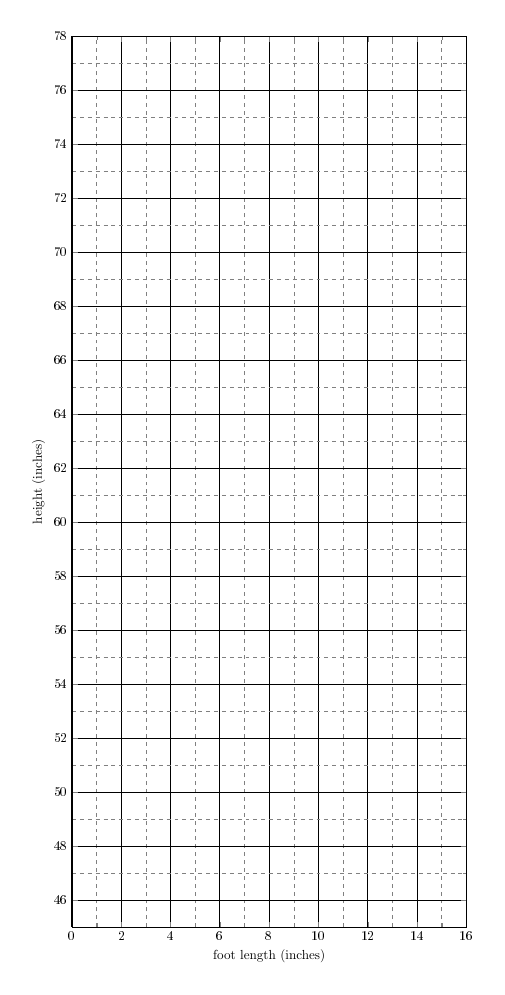
\begin{tikzpicture}[scale=0.475]
        \begin{axis}[
            xmin = 0, xmax = 16,
            ymin = 45, ymax = 78,
            % xtick distance = 2.5,
            % ytick distance = 0.5,
            grid = both,
            minor tick num = 1,
            major grid style = {thick,black},
            minor grid style = {dashed,black!50},
            width = \textwidth,
            height = 10in,
            xlabel = {foot length (inches)},
            ylabel = {height (inches)},
            legend cell align = {left},
        ]
        \end{axis}
    \end{tikzpicture}

\end{minipage}

\begin{enumerate}[fullwidth,label={\Large$\bm{\square}$}\,\arabic*.,resume]
    \item How would the scatterplot change if the order of the points in the table 
        were reversed? \hrulefill 
        \begin{itemize}
            \item[]\hrulefill 
            \item[]\hrulefill 
        \end{itemize} 
    \item The term ``outlier'' refers to points on a scatterplot that are 
        far away from the line of best fit. 
        If there are just a few of these, they can sometimes be explained by 
        human errors in the measurement process. 
        \begin{itemize}
            \item How many outliers do you see in the scatterplot? \underline{\hspace{0.5in}}
            \item Describe at least two errors could create outliers in this activity?
            \item[]\hrulefill
            \item[]\hrulefill
            \item[]\hrulefill
            \item[]\hrulefill
        \end{itemize}
    \item There is actually something ``odd'' about the $(x,y)$ scatterplot grid  
        on the last page. 
        \begin{itemize}
            \item What are the coordinates of the point in the lower-left corner of the grid?
                $(x,y) = $ (\underline{\hspace{1em}},\underline{\hspace{1em}})
            \item Explain what is ``odd'' about this. \hrulefill
            \begin{itemize}
                \item[]\hrulefill
                \item[]\hrulefill
                \item[]\hrulefill
            \end{itemize}        \end{itemize} 
\end{enumerate}

\subsection*{Line of Best Fit}

\begin{enumerate}[fullwidth,label={\Large$\bm{\square}$}\,\arabic*.,resume]
    \item Which shape do you think ``best fits'' the dots? (circle one)
        \begin{tcbraster}[
            raster equal height, raster columns = 3,
            raster left skip = 0.3in, raster right skip = 0.3in, raster column skip = 0.2in,
            colback=white, valign=center,
        ]
            \begin{tcolorbox}
                \centering
                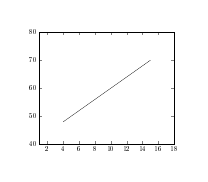
\begin{tikzpicture}[scale=0.25]
                    \begin{axis}[
                        ymin = 40, ymax = 80,
                        xmin = 1, xmax = 18]
                        \addplot[domain = 4:15,] {2*x + 40};
                    \end{axis}
                \end{tikzpicture}\\
                \myEmph{Linear}\\
                $y = mx+b$
            \end{tcolorbox}
            \begin{tcolorbox}
                \centering
                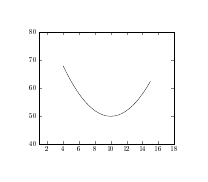
\begin{tikzpicture}[scale=0.25]
                    \begin{axis}[
                        ymin = 40, ymax = 80,
                        xmin = 1, xmax = 18]
                        \addplot[domain = 4:15,] {0.5*(x-10)^2+50.0};
                    \end{axis}
                \end{tikzpicture}\\
                \myEmph{Quadratic}\\
                $y = ax^2 + bx + c$
            \end{tcolorbox}
            \begin{tcolorbox}
                \centering
                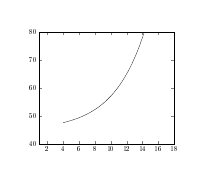
\begin{tikzpicture}[scale=0.25]
                    \begin{axis}[
                        ymin = 40, ymax = 80,
                        xmin = 1, xmax = 18]
                        \addplot[domain = 4:15,] {exp(0.25*x)+45};
                    \end{axis}
                \end{tikzpicture}\\
                \myEmph{Exponential}\\
                $y = ae^{bx}$
            \end{tcolorbox}
        \end{tcbraster}
    \item Use a ruler to draw a \myEmph{line of best fit} that you think almost goes through all the points.
    \item Estimate the \myEmph{slope} and \myEmph{$\bm{y}$-intercept} for your line.
        \begin{itemize}
            \item slope:
                \begin{itemize}
                    \item two points on your line: 
                        $(x_1,y_1) = $ (\underline{\hspace{4em}},\underline{\hspace{4em}})
                        $(x_2,y_2) = $ (\underline{\hspace{4em}},\underline{\hspace{4em}})
                    \item {\itshape my estimated} 
                        $m = \frac{\Delta y}{\Delta x} = \frac{y_2 - y_1}{x_2 - x_1} =$ 
                        \underline{\hspace{3in}}
                \end{itemize}
            \item $y$-intercept:
                \begin{itemize}
                    \item Where does your line cross the $y$-axis?
                    \item {\itshape my estimated} $b =$ \underline{\hspace{1in}}
                \end{itemize}
        \end{itemize}
    \item Wiggle the ruler a tiny amount so you get a {\itshape slightly different} line.
        \begin{itemize}
            \item When you do that, how much does the $y$-intercept, $b$, change?
                \underline{\hspace{0.5in}}
            \item The term ``sensitivity'' refers to when the value of a variable 
                changes ``a lot'' when something else changes. 
                Is $b$ sensitive to small changes in your ruler? 
                Explain why or why not. \hrulefill
                \begin{itemize}[fullwidth]
                    \item[] \hrulefill 
                    \item[] \hrulefill 
                \end{itemize}
        \end{itemize}
    \item Do you think there is a {\itshape physical interpretation} of 
        the $y$-intercept, $b$? Explain why or why not. \hrulefill 
        \begin{itemize}
            \item[] \hrulefill 
            \item[] \hrulefill 
            \item[] \hrulefill 
        \end{itemize}
\end{enumerate}

\subsection*{Linear Regression Analysis}

\begin{enumerate}[fullwidth,label={\Large$\bm{\square}$}\,\arabic*.,resume]
    \item Open the {\scshape Desmos} graphing calculator on your phone, or share with someone else.
    \item Create an empty {\scshape Desmos} $(x_1,y_1)$ \myEmph{table} by clicking on \fbox{\Large +}.
    \item Enter at least \myEmph{15 rows} from your table on the next page into the {\scshape Desmos} table.
        \begin{itemize}
            \item Put {\itshape foot length} data into the $x_1$ column.
            \item Put {\itshape height} data into the $y_1$ column.
            \item How many rows did you copy? \underline{\hspace{1in}}
            \item How many dots do you see in the {\scshape Desmos} scatterplot? \underline{\hspace{1in}}
        \end{itemize}
    \item Tell {\scshape Desmos} to do a \myEmph{linear regression} 
        to find the ``best fit'' line for the scatterplot.
        Do this by entering the following formula into {\scshape Desmos}.
        \begin{itemize}
            \item {\ttfamily y1 \raisebox{0.25em}{\large\texttildelow}\, m x1  +  b}
        \end{itemize}
    \item Write down the values of $m$ and $b$ that {\scshape Desmos} calculated.
        \begin{itemize}
            \item {\scshape Desmos} $m =$ \underline{\hspace{0.5in}}
            \item {\scshape Desmos} $b =$ \underline{\hspace{0.5in}}
        \end{itemize}
\item Compare the values of $m$ and $b$ that {\scshape Desmos} calculated 
        to your values in step 9, above. What do you notice?
        \begin{itemize}
            \item How my slope estimate compared to {\scshape Desmos}: \hrulefill
            \item[] \hrulefill
            \item[] \hrulefill
            \item How my $y$-intercept estimate compared to {\scshape Desmos}: \hrulefill
            \item[] \hrulefill
            \item[] \hrulefill
        \end{itemize}
\end{enumerate}



\end{document}